\documentclass[10pt,a4paper]{article}
\usepackage{times}                       % 使用 Times New Roman 字体
\usepackage{xeCJK}         % 中文支持宏包
\usepackage{color}                       % 支持彩色

\usepackage{comment}
\usepackage{amsmath}
\usepackage{amssymb}
\usepackage{amsthm}
\usepackage{amscd}
\usepackage{graphicx}
\usepackage{indentfirst}
\usepackage{titlesec}
\usepackage[top=25.4mm, bottom=25.4mm, left=31.7mm, right=32.2mm]{geometry}

%页面设置
%\begin{CJK*}{GBK}{hei}
%\theoremstyle{definition}
%\newtheoremstyle{mythm}{1.5ex plus 1ex minus .2ex}{1.5ex plus 1ex minus .2ex}
%   {\kai}{\parindent}{\song\bfseries}{}{1em}{}
\newtheoremstyle{mythm}{1ex}{1ex}%定理环境的上下间距.
{\CJKfamily{song}}{\parindent}{\CJKfamily{hei} \bf}{}{1em}{}%定理内容为宋体, 缩进, 定理名称为黑粗体
\theoremstyle{mythm}%设置定理环境
\newtheorem{thm}{定理~}[section]
\newtheorem{lem}[thm]{引理~}
\newtheorem{pro}[thm]{性质~}
\newtheorem{fact}[thm]{Fact}
\newtheorem{prop}[thm]{命题~}
\newtheorem{ques}[thm]{问题~}
\newtheorem{cor}[thm]{推论~}
\newtheorem{de}[thm]{定义~}
\newtheorem{rem}[thm]{注记~}
\numberwithin{equation}{section}
%\end{CJK*}
\renewcommand\refname{\CJKfamily{hei}}
%\renewcommand{\abstractname}{摘要}
%%%%%%%%%%%%%%%%下面几行用于改变证明环境的定义
\makeatletter
\renewenvironment{proof}[1][\proofname]{\par
\pushQED{\qed}%
\normalfont \topsep6\p@\@plus6\p@ \labelsep1em\relax
\trivlist
\item[\hskip\labelsep\indent
\bfseries #1]\ignorespaces
}{%
\popQED\endtrivlist\@endpefalse
}
\makeatother
%%%%%%%%%%%%%%(http://latex.yo2.cn)
\renewcommand{\proofname}{\CJKfamily{hei}证明}

\renewcommand{\thefootnote}{\fnsymbol{footnote}}
%\titleformat{\section}{\CJKfamily{hei} }{\arabic{section}{1em}{}
\titleformat{\section}{\large \bf \CJKfamily{hei} }{{\bf \thesection\space}}{0pt}{}

\begin{document}
%\setlength{\baselineskip}{1ex}%设置行距
\setlength{\abovedisplayskip}{1ex} %设置公式上边间距
\setlength{\belowdisplayskip}{1ex} %设置公式下边间距
%\begin{CJK*}{GBK}{song}

\author{马国芳11621003}                                 % 作者
\title{计算机应用数学实验报告}              % 题目
\maketitle                                           % 生成标题

\section{引言}
根据在应用数学课堂上学习的知识,使用 python 语言实现了前五个作业的要求:多项式拟 合、PCA、GMM、LM 算法和 SVM 的实现。开发工具为pyCharm,语言为python。使用的库有 numpy、scipy、 matplotlib 等。通过对 PCA、SVM、GMM 等方法的实现,对这些知识点有了更深刻的认识。文本将对实现过程中用到的方法思想进行简单介绍。
\section{实验方法及结果}
\subsection{homework1}
我们有一条需要拟合的曲线$t(x)$,现在我们观察到了这条曲线上的n个点:
$$[(x_1,t(x_1)),(x_2,t(x_2)...(x_n,t(x_n))]$$
接下来我们要用一条多项式曲线
$$y(x,w)=w_0+w_1x+w_2x_2+...w_Mx_M$$
来拟合$t(x)$。最小二乘就是要最小化误差函数:
$$E(w)=\sum_{i=1}^n(y(x_i,w)-t(x_i))^2$$
我们的$t(x)$选为$ sin(2\Pi x)$,并加上一个正态分布的小噪音干扰。然后用多项式分布去拟合。
接下来我们应该是要加上penalty term来控制过拟合的情况。误差函数变为了
$$E(w)=\sum_{i=1}^n(y(x_i,w)-t(x_i))^2+\lambda ||w||^2$$

 \paragraph{实验结果}实验结果如下图所示:

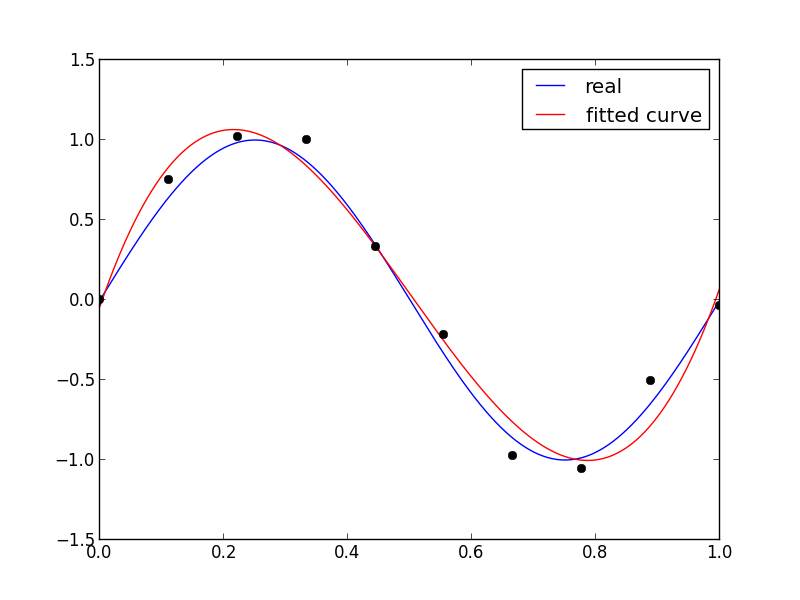
\includegraphics[height=2in]{figure1-1.png} 

图1-1 sample the function curve of y = sin(2πx) with Gaussian noise

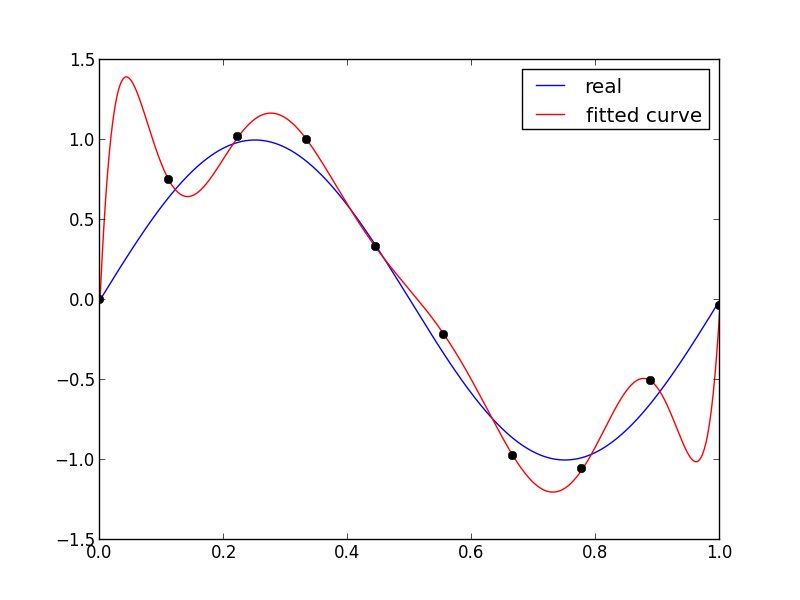
\includegraphics[height=2in]{figure1-2.png} 

图1-2fit degree 3 and 9 curves in 10 samples

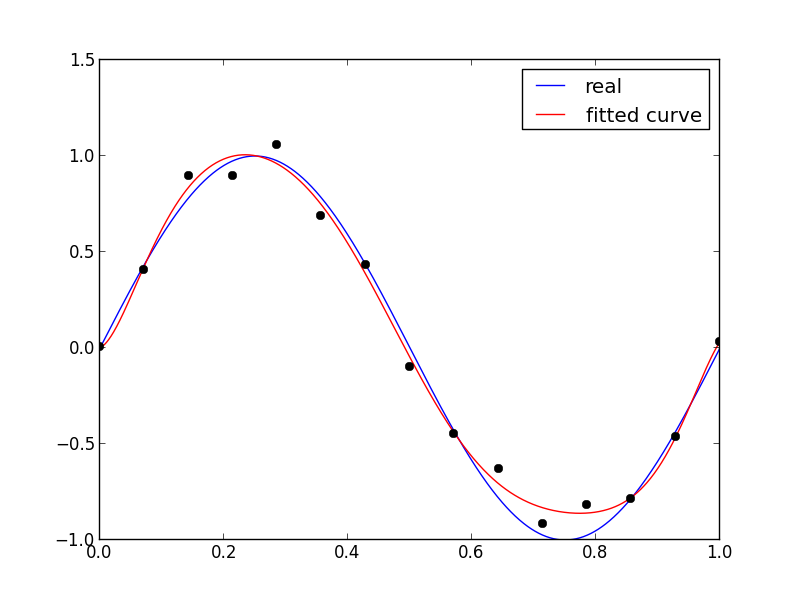
\includegraphics[height=2in]{figure1-3.png} 
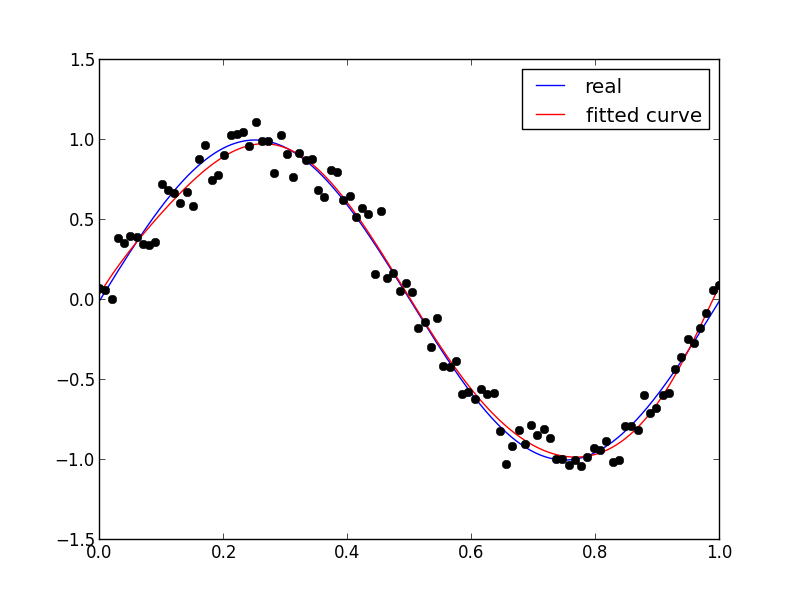
\includegraphics[height=2in]{figure1-4.png} 

图1-3 fit degree 9 curves in 15 (left)and 100(right) samples

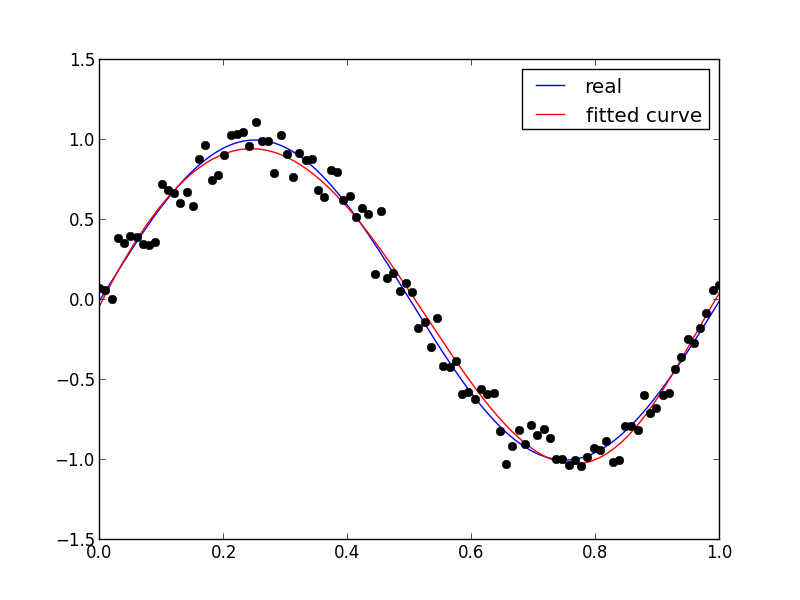
\includegraphics[height=2in]{figure1-5.png} 

图1-4 fit degree 9 curve in 10 samples but with regularization term

\subsection{homework2}
主成份分析的目的是:寻找最小均方意义下, 最能代表原始数据的投影方法。主要用于特征的降维。PCA的主要思想是寻找到数据的主轴方 向,由主轴构成一个新的坐标系,这里的维数可以比原维数低,然后数据由原坐标系向新的坐 标系投影,这个投影的过程就可以是降维的过程。

算法的步骤:

1.计算所有样本的均值$m$和散布矩阵$S$,所谓散布矩阵同协方差矩阵;

2.计算$S$的特征值,然后由大到小排序;

3.选择前$n′$个 特征值对应的特征矢量作成一个变换矩阵$E = [e1, e2, ,, en.]$;

4.最后,对于之前每一个$n$维的特 征矢量$x$可以转换为$n$.维的新特征矢量$y$:

$$y=transpose(E)(x-m)$$

 \paragraph{实验结果}实验结果如下图所示:
 
 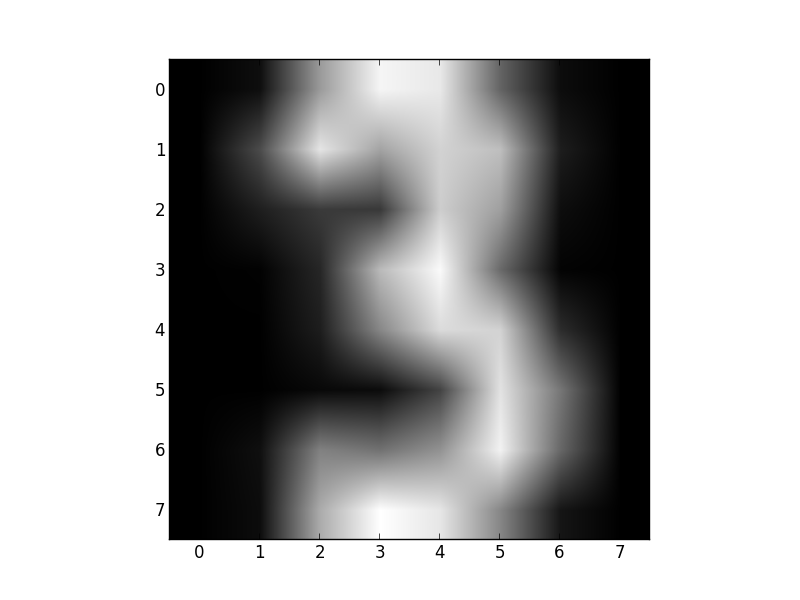
\includegraphics[height=2in]{figure2-1.png} 
 
 图2-1  所有’3’的均值图
 
 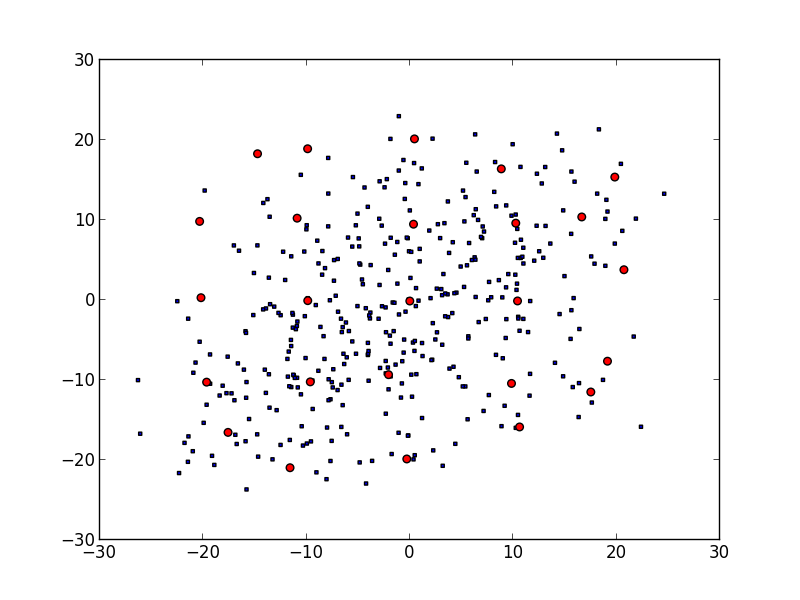
\includegraphics[height=2in]{figure2-2.png} 
 
 图2-2  PCA降维后每个’3’的分布图
 
  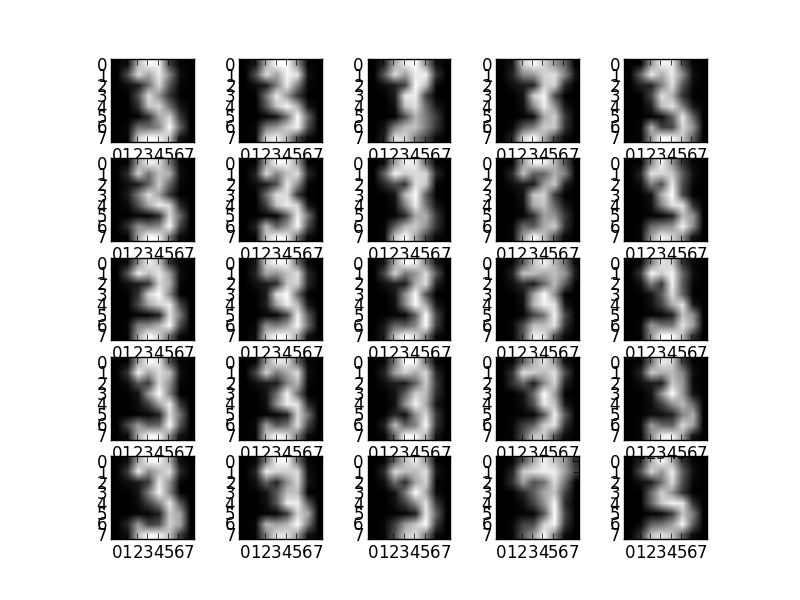
\includegraphics[height=2in]{figure2-3.png} 
  
图2-2  PCA降维后’3’的图像


\subsection{homework3}
这个试验中主要学习了多维高斯模型的生成及 EM 算法。在多维高斯模型生成过程中,首先 生成一个二维的标准正态分布 N,生成的正态分布为$MN=N*\sum^{1/2}+\mu$
。然后采用 EM 算法 求解各高斯分布的参数及其对应的比例。程序中定义了多个函数用于生成数据 (采用的方法即为 PPT 上的思想)、生成高斯混合模型、EM 算法 (E 步和 M 步)
 \paragraph{实验结果}实验结果如下图所示:
 
 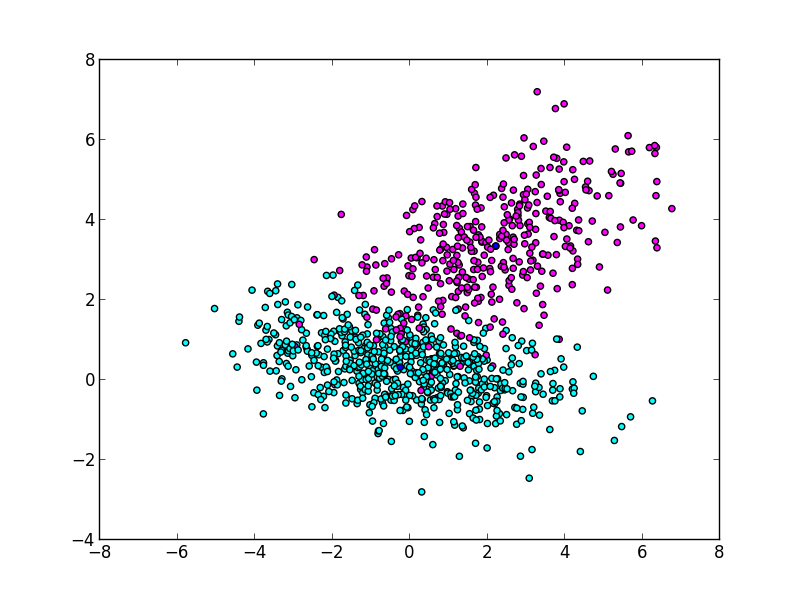
\includegraphics[height=2in]{figure3-1.png} 
 
图3-1  随机生成的二维高斯分布

 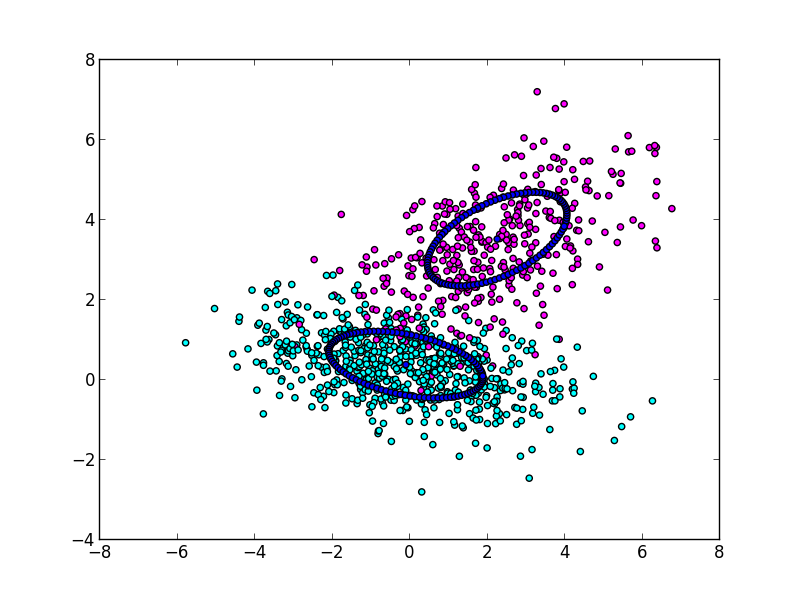
\includegraphics[height=2in]{figure3-2.png} 
 
图3-2 MOG聚类后的结果
\subsection{homework4}

该算法是使用最广泛的非线性最小二乘算法。它是利用梯度求最大(小) 值的算法。它同时具有梯度法和牛顿法的优点。当λ很小 时,步长等于牛顿法步长,当λ很大时,步长约等于梯度下降法的步长。LM算法的实现的关键 是用模型函数f 对待估参数向量p在其领域内做线性近似,忽略掉二阶以上的导数项,从而转化 为线性最小二乘问题,它具有收敛速度快等优点。LM算法属于一种“信赖域法”,所谓的信赖 域法,即是:在最优化算法中,都是要求一个函数的极小值,每一步迭代中,都要求目标函数 值是下降的,而信赖域法,顾名思义,就是从初始点开始,先假设一个可以信赖的最大位移s, 然后在以当前点为中心,以s为半径的区域内,通过寻找目标函数的一个近似函数(二次的)的 最优点,来求解得到真正的位移。在得到了位移之后,再计算目标函数值,如果其使目标函数 值的下降满足了一定条件,那么就说明这个位移是可靠的,则继续按此规则迭代计算下去;如 果其不能使目标函数值的下降满足一定的条件,则应减小信赖域的范围,再重新求解。

 \paragraph{实验结果}实验结果如下图所示:
 
 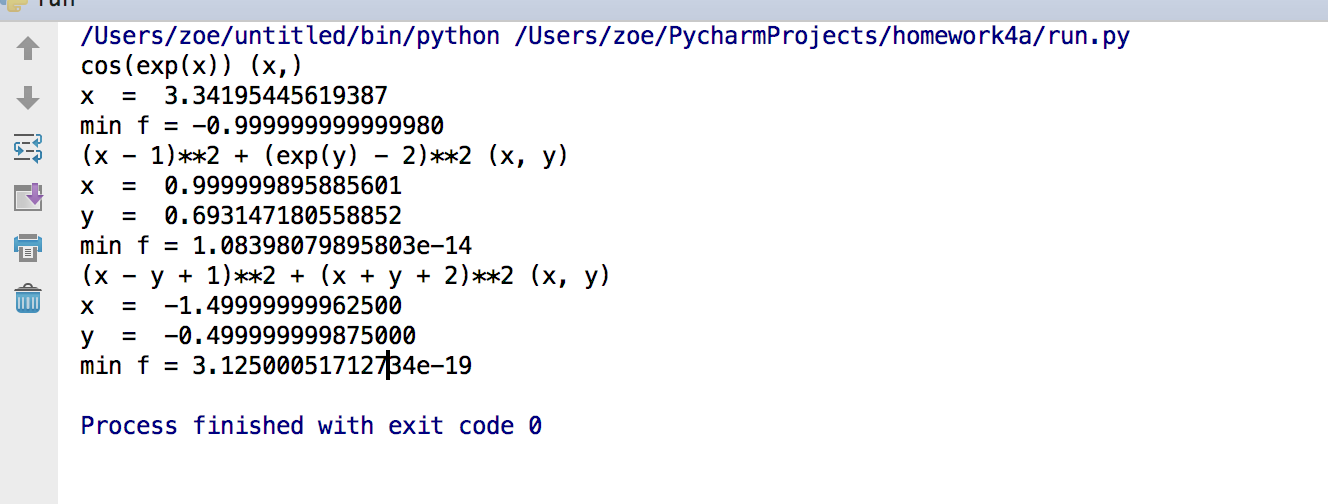
\includegraphics[height=2in]{figure4.png} 
 
图4  LM后收敛的结果




\subsection{homework5}

1、数据的定义。根据作业要求,在 testData.txt 中定义了 100 个数据,每个数据都是二 维的,并且包含自己的 label。整体数据分为两类,label 为 1 和 -1。前 80 个数据用于训练,后 20 个数据用于测试。
2、SVM训练过程。SVM 试图找一个超平面来对样本进行分割,这是一个凸二次规划问题,具有全局最优解,本次实验使用的优化算法为 SMO 算法,将大的优 化问题分解成多个小问题。主要的思想是不断重复的选择两个拉格朗日乘子,固定其他的乘子 进行优化,并根据优化后的乘子更新截距 b 的值,直到收敛 (也就是所有变量都满足了 KTT 条 件)。核函数选用线性函数。定义 SVM 的数据结构,包含训练集、每个样本的拉格朗日乘子、核 矩阵等信息。python 其实是一种面向对象的编程语言,根据要实现的功能定义了多个函数。包 括选择第二个拉格朗日乘子,对两个乘子进行优化,主要的训练过程,测试训练好的 SVM 模型
以及对最终分类结果的显示。
3、主控制。主控制程序主要分四步:读取数据,训练数据,测试数据,显示结果。后三步都可以直接调用 SVM 中定义的函数来实现。

 \paragraph{实验结果}本实验随机生成了一些测试点,对它们进行SVM分类。分类的结果如图所示:
 
 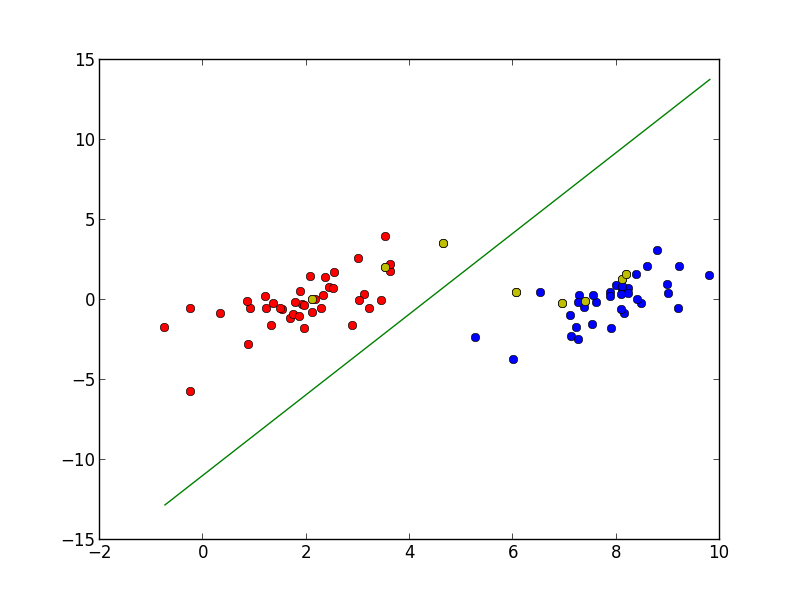
\includegraphics[height=2in]{figure5-2.png} 
 
图5-1  SVM分类后的结果

 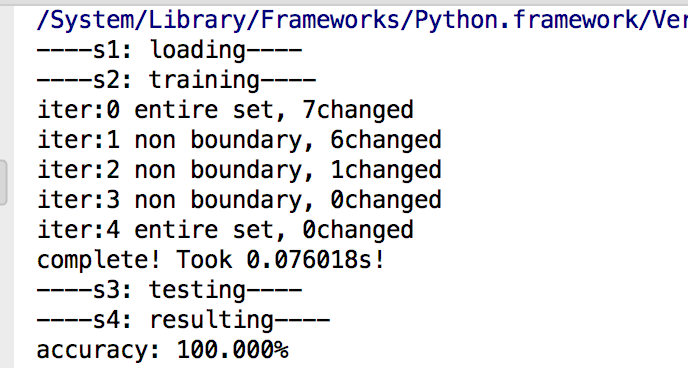
\includegraphics[height=2in]{figure5-1.png} 
 
图5-1  程序结果截图
\section{小结与讨论}
本次实验通过python来实践了几个经典的算法。在实现这些算法的过程中,尽量避免了使用
一些现成的工具库,从原理出发,对应用数学中一些算法的原理有了更深入的认识。

通过实现了这五个作业,不仅对课堂上学到的知识有了更深刻的认识,同时让自己接触到了 一门以前没有用过的语言,提高了自己的编程水平。自己在平时也看了一些自己研究领域的文 章,深刻感受到应用数学课上介绍的数学知识还是非常有用的,与自己正在做的东西息息相关。 虽然每周二晚上上三个小时的数学课还是很累的,但是在对自己的科研还是很有帮助的。痛并 快乐着。

\begin{thebibliography}{MM}
\addtolength{\itemsep}{-0.5em}
\begin{small}

\end{small}
\end{thebibliography}
\newpage
%\end{CJK*}
\end{document}

